\chapter{Determinants}\label{chapter:determinants}

\section{Commutative Rings}

In this chapter, we define determinants, and we do so for a broader range of matrices, in which its entries are not only from a field but of a more general form, such as polynomials. To do that, we need the following definition.

\begin{definition}[Ring]
	A \textbf{ring}	is a set $K$ together with two operations $+$ (addition) and $\cdot$ (multiplication) satisfying:
	\begin{enumerate}
		\item $K$ is a commutative group under addition;
		\item Multiplication is associative: $(x \cdot y) \cdot z = x \cdot (y \cdot z)$;
		\item The two distributive laws hold: $x \cdot (y + z) = x \cdot y + x \cdot z$ and $(y + z) \cdot x = y\cdot x + z \cdot x$.
	\end{enumerate}
	
	If $x \cdot y = y \cdot x$, then the ring $K$ is said to be \textbf{commutative}.
	
	If there exists an element $e \in K$ such that $e \cdot x = c \cdot e = x$ for each $x \in K$, then $e$ is called the \textbf{identity} for $K$ and the ring $K$ is said to be a \textbf{ring with identity}.
\end{definition}

In this text, we use `ring' to denote a commutative ring with identity.

\section{Determinant Functions}

Intuitively, the determinant has a geometrical meaning: it is an oriented volume. What do we mean by that? \footnote{For more information on the geometrical interpretation of the determinant, please refer to \cite{dieudonne1969linear}.}

Consider a matrix $A$ and $T_A$ is the transformation that $A$ represents. Notice that the standard basis is a unitary cube, which we denote by $C$. We obtain a parallelepiped by applying the transformation $T_A$ to the unitary cube $C$ (i.e., the standard basis).

So the determinant is the volume of the parallelepiped obtained by the range of the unitary cube by the transformation represented by the matrix.

\begin{figure}[h]
	\centering
	  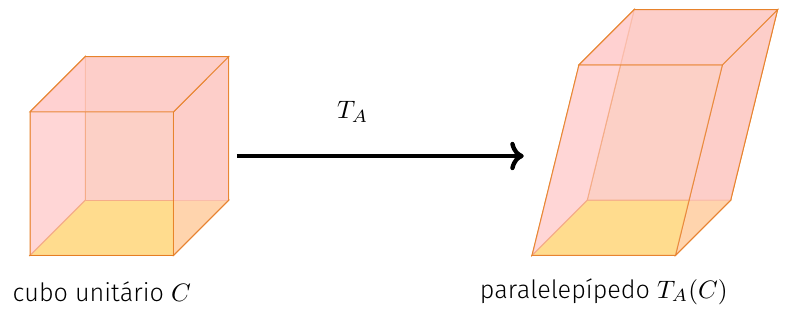
\includegraphics[width=0.8\textwidth]{Figures/geometria_determinante.png} 
	  \caption{The unitary cube $C$ mapped into the parallelepiped $T_A(C)$ \cite{miranda2020avancada}.}
	  \label{fig:geometry-determinant}
\end{figure}

% What properties does this volume must have?

% Volume function: from the square matrices to the field satisfying two simple properties.

% Proposition:

% 1. If a column is zero, then the volume is zero. 

% 2. If the columns are L.D., then the volume is zero.

% 3. Inverting two columns renders $(-1)$ times the original volume. I.e. the volume is alternating (think about permutation groups). 

% 4. Volume is linear in each entry of the matrix (the volume is multilinear).

% Alternating fails at fields of characteristic two. Better way: if two columns are equal, then the volume is zero. Is equivalent to the previous definition and works at $\text{char} ~\mathbb{F} = 2$.

% Theorem: A function is a volume volume iff.

% 1. Multilinear;

% 2. Alternating;

% Definition: a function is said to be a determinant if.

% 1. Multilinear;

% 2. Alternating;

% 3. Volume of the unitary cube is one.

% Theorem: uniqueness of the determinant.

Algebraically, our goal is to define a function $\textbf{M}_n(K) \longrightarrow K$ such that it is linear in each row of the matrix (hence it is zero if two rows are equal), and the value of this function applied to the identity matrix is one.

\begin{definition}[$n$-linear]
	Let $K$ be a ring, $n$ a positive integer, and let $D$ be the following function
	\begin{equation*}
		\begin{aligned}
			D : \textbf{M}_n(K) &\longrightarrow K \\
			A &\longmapsto D(A)
		\end{aligned}
	\end{equation*}
	
	Then $D$ is called \textbf{n-linear} if for each $i$, $1 \leq i \leq n$, $D$ is a linear function of the $i$th row when the other $(n-1)$ rows are held fixed.
\end{definition}

Notice that if $v_1, \ldots, v_n$ are the rows of $A$,
\[
	A = \begin{bmatrix}
		\rule{0.7cm}{0.01cm} && v_1 && \rule{0.7cm}{0.01cm} \\
		\rule{0.7cm}{0.01cm} && v_2 && \rule{0.7cm}{0.01cm} \\
		&& \vdots && \\
		\rule{0.7cm}{0.01cm} && v_n && \rule{0.7cm}{0.01cm} \\
	\end{bmatrix}
\]	
Then $D(A)$ is a function of the rows of $A$, i.e.
\[
	D(A) = D(v_1, v_2, \ldots, v_n)
\]

Then $D$ is $n$-linear means that
\[
	D(v_1, \ldots, cv_i + v_i', \ldots, v_n) = cD(v_1, \ldots, v_i, \ldots, v_n) + D(v_1, \ldots, v_i', \ldots v_n)
\]

\begin{example}
	The product of the diagonal entries of an $n \times n$ matrix is $n$-linear.
\end{example}

\begin{lemma}
	A linear combination of $n$-linear functions is $n$-linear.
\end{lemma}

\begin{proof}
	Let $D, E$ be $n$-linears. If $a, b \in K$, then 
	\[
		(aD + bE)(A) = aD(A) + bE(A)
	\]

	Fixing all rows except the $i$th row, we can write $D(v_i)$ instead of $D(A)$. Then 
	\begin{equation*}
		\begin{aligned}
			(aD + bE)(cv_i + v_i') &= aD(cv_i + v_i') + bE(cv_i + v_i') \\
								   &= acD(v_i) + aD(v_i') + bcE(v_i) + bE(v_i') \\
								   &= c(aD + bE)(v_i) + (aD+bE)(v_i')
		\end{aligned}
	\end{equation*}
\end{proof}

\begin{example}
	By the above lemma, the function $D(A) = A_{11}A_{22} - A_{12}A_{21}$ is $2$-linear. 
\end{example}

Notice that for the $D$ defined in the preceding example, we have
\begin{itemize}
	\item $D(I) = 1$;
	\item If two rows are equal, then $D(A) = 0$; 
	\item If $A'$ is obtained from $A$ by interchanging its rows, then $D(A') = - D(A)$, since \[ D(A') = A_{11}'A_{22}' - A_{12}'A_{21}' = A_{21}A_{12} - A_{22}A_{11} = -D(A) \]
\end{itemize}

This fact (plus the geometrical interpretation of volume) induces the following nomenclature.

\begin{definition}[Alternating]
	Let $D$ be a $n$-linear function. We say that $D$ is \textbf{alternating} (or \textbf{alternated}) if the following two conditions are satisfied:
	\begin{enumerate}
		\item $D(A) = 0$ whenever two rows of $A$ are equal;
		\item $D(A') = -D(A)$ if $A'$ is a matrix obtained from $A$ by interchanging two rows of $A$.
	\end{enumerate}
\end{definition}

Notice that the second condition fails at fields of characteristic two. But actually, nothing is lost! In fact, the first condition implies the second one. Therefore, we can define alternating functions just using the first condition, which will be equivalent to the previous definition and works at $\text{char} ~\mathbb{F} = 2$.

With these tools at hand, we can finally define the determinant.

\begin{definition}[Determinant]
	Let $K$ be a ring, and $n$ a positive integer. Suppose that $D : \textbf{M}_n(K) \longrightarrow K$. Then $D$ is said to be a \textbf{determinant function} if $D$ is $n$-linear, alternating and $D(I) = 1$.
\end{definition}

Our task now is to show the existence and uniqueness of the determinant function.

For $n = 1$, it is trivial: $A = [a]$ and $D(A) = a$.

In the case $n=2$, $D(A)$ is of the form
\[
	D(A) = D(A_{11}e_1 + A_{12}e_2, A_{21}e_1 + A_{22}e_2)
\]

If $D$ is $2$-linear, we have that
\begin{equation*}
	\begin{aligned}
		D(A) &= A_{11}D(e_1, A_{21}e_1 + A_{22}e_2) + A_{12}D(e_2, A_{21}e_1 + A_{22}e_2) \\
		&= A_{11} A_{21} D(e_1, e_1) + A_{11} A_{22} D(e_1, e_2) + A_{12} A_{21} D(e_2, e_1) + A_{12} A_{22} D(e_2, e_2)
	\end{aligned}
\end{equation*}

Hence, $D$ is completely determined by
\[
	D(e_1, e_1), ~D(e_1, e_2), ~D(e_2, e_1), \text{ and } D(e_2, e_2)
\]

We've shown that $D(A) = A_{11}A_{22} - A_{12}A_{21}$ is a determinant function. By the preceeding argument, then $D$ is also unique.

Since $D$ is alternating, 
\[
	D(e_1, e_1) = D(e_2, e_2) = 0
\]
and
\[
	D(e_2, e_1) = - D(e_1, e_2) = -D(I)
\]
and $D(I) = 1$.

\begin{example}
	Let $D$ be any alternating $3$-linear function on $3 \times 3$ matrices over the polynomial ring $\mathbb{F}[x]$. And let
	\[
		A = \begin{bmatrix}
			x && 0 && -x^2 \\
			0 && 1 && 0 \\
			1 && 0 && x^3
		\end{bmatrix}
	\]

	Then $D(A) = D(xe_1 - x^2 e_3, e_2, e_1 + x^3e_3)$. Since $D$ is linear in each row,
	\begin{equation*}
		\begin{aligned}
		D(A) &= xD(e_1, e_2, e_1 + x^3 e_3) - x^2D(e_3, e_2, e_1 + x^3 e_3) \\
		&= xD(e_1, e_2, e_1) + x^4D(e_1, e_2, e_3) - x^2D(e_3, e_2, e_1) - x^5D(e_3, e_2, e_3)
		\end{aligned}
	\end{equation*}

	By the hypothesis that $D$ is alternating it follows that
	\[
		D(A) = (x^4 + x^2)D(e_1, e_2, e_3)
	\]
\end{example}

\begin{lemma}
	Let $D$ be a $2$-linear function such that $D(A) = 0$ for all $2 \times 2$ matrices $A$ having equal rows. Then $D$ is alternating.
\end{lemma}

\begin{proof}
	We show that if $A=(u,v)$, then $D(v,u) = -D(u,v)$. Since $D$ is $2$-linear,
	\[
		D(u+v, u+v) = D(u,u) + D(u,v) + D(v,u) + D(v,v) = 0
	\]

	Hence,
	\[
		0 = D(u,v) + D(v,u)
	\]
\end{proof}

\begin{lemma}
	If $D$ is an $n$-linear function and $D(A) = 0$ whenever two adjacent rows of $A$ are equal, then $D$ is alternating.
\end{lemma}

\begin{proof}
	If $A'$ is obtained by interchanging two adjacent rows of $A$, then by the preceeding lemma, $D(A') = -D(A)$. 

	We need to show that $D(A) = 0$ when any two rows of $A$ are equal. Let $B$ be the matrix obtained by interchanging rows $i$ and $j$ of $A$, where $i < j$. We obtain $B$ by a succession of interchanges of pairs of adjacent rows.

	First we interchange the rows $i$ and $i+1$ until the rows are in the order
	\[
		v_1, \ldots, v_{i-1}, v_{i+1}, \ldots, v_j, v_i, v_{j+1}, \ldots, v_n
	\]
	
	This process required $k = j-i$ interchanges of adjacent rows. Now, we need to move $v_j$ to the $i$th position, requiring more $j-1-i = k-1$ interchanges of adjacent rows.

	Since we obtained $B$ from $A$ by $k+(k-1) = 2k-1$ interchanges,
	\[
		D(B) = (-1)^{2k-1}D(A) = -D(A)
	\]

	Now let $A$ be a matrix with two equal rows, say $v_i = v_j$, where $i < j$.
	
	If $j = i+1$, then $D(A) = 0$, since $A$ has two equal and adjacent rows.

	If $j > i+1$, then the batrix $B$, obtained by exchanging the rows $j$ and $i+1$ of the matrix $A$ has two equal and adjacent rows. I.e., $D(B) = 0$.

	Since $D(A) = -D(B)$, then it follows that $D(A) = 0$.
\end{proof}

The next definition and theorem will be applied when we study the cofactor method.

\begin{definition}
	If $n>1$ and $A$ is an $n \times n$ matrix, let $A(i|j)$ denote the $(n-1) \times (n-1)$ matrix obtained by deleting the $i$th row and the $j$th row column of $A$. 

	If $D$ is an $(n-1)$-linear function, then we define $D_{ij}(A) = D[A(i|j)]$.
\end{definition}

\begin{theorem}\label{thm:cofactor-prep}
	Let $n>1$ and $D$ an alternating $(n-1)$-linear function on $(n-1) \times (n-1)$ matrices. For each $j$, where $1 \leq j \leq n$, the function $E_j$ defined by
	\[
		E_j(A) = \sum_{i=1}^n (-1)^{i+j} A_{ij} D_{ij}(A)
	\]
	is an alternating $n$-linear function on $n \times n$ matrices $A$. If $D$ is a determinant function, so is each $E_j$.
\end{theorem}

\begin{proof}
	\textbf{First step:} Show that $E_j$ is $n$-linear.
	
	Notice that $D_{ij}(A)$ is independent of the the $ith$ row of $A$. Since $D$ is $(n-1)$-linear, it is linear as a function of any row except row $i$. Therefore $A_{ij} D_{ij}(A)$ is an $n$-linear function of $A$. Hence, $E_j$ is $n$-linear.	
	
	\textbf{Second step:} Show that $E_j$ is alternating.
	
	Suppose that two adjacent rows $a_k$ and $a_{k+1}$ are equal. If $i \neq k$ and $i \neq k+1$, then $A(i|j)$ has two equal rows, and $D_{ij}(A) = 0$. Therefore,
	\[
		E_j(A) = (-1)^{k+j} A_{kj}D_{kj}(A) + (-1)^{k+1+j} A_{(k+1)j} D_{(k+1)j}(A)
	\]
	
	Using that $a_k = a_{k+1}$,
	\[
		A_{kj} = A_{(k+1)j} \text{ and } A(k|j) = A(k+1|j)
	\]
	
	Therefore,
	\[
		D_{kj}(A) = D[A(k|j)] = D[A(k+1|j)] = D_{(k+1)j}(A)
	\]
	which implies that $E_j(A) = 0$. Hence, $E_j(A) = 0$ whenever $A$ has two equal and adjacent rows. I.e., $E_j$ is alternating.
	
	\textbf{Third step:} Show that $E_j(I) = 1$.
	
	Suppose that $D$ is a determinant function. Then
	\[
		E_j(I_n) = D(I_{n-1}) = 1 \implies E_j(I_n) = 1
	\]
	
	Hence, $E_j$ is a determinant function.
\end{proof}

\begin{corollary}
	If $K$ is a ring and $n$ is a positive integer, then there exists at least one determinant function on $\textbf{M}_n(K)$.
\end{corollary}

\section{Permutations and the Uniqueness of Determinants}

To prove the uniqueness of the determinant function, we proceed in steps. Here, suppose that $A$ is an $n \times n$ matrix over $K$ and $D$ is an alternanting $n$-linear function on these matrices.

\textbf{First step.} Express every row $a_1, a_2, \ldots, a_n$ of the matrix $A$ in terms of the standard basis $e_1, e_2, \ldots, e_n$.

\textbf{Second step.} Using multilinearity, express $D(A)$ as a linear combination of the matrix entries and the determinant of the standard vectors.

To do that, notice that, for $1 \leq i \leq n$, each row can be expressed as
\[
	a_i = \sum_{j=1}^n A(i,j)e_j
\]

Hence,
\begin{equation*}
	\begin{aligned}
		D(A) &= D\left( \sum_{j=1}^n A(i,j)e_j, a_2, \ldots, a_n \right) \\
			 &= \sum_{j=1}^n A(1,j)D(e_j, a_2, \ldots, a_n)
	\end{aligned}
\end{equation*}

Replacing $a_2$ by $\sum_{k=1}^n A(2,k)e_k$, 
\begin{equation*}
	\begin{aligned}
		D(e_j, a_2, \ldots, a_n) &= \sum_{k=1}^n A(2,k)D(e_j, e_k, \ldots, a_n)
	\end{aligned}
\end{equation*}

Thus,
\begin{equation*}
	\begin{aligned}
		D(A) = \sum_{j,k}A(1,j)A(2,k)D(e_j, e_k, \ldots, a_n)
	\end{aligned}
\end{equation*}

Repeating this process, we obtain an important expression for $D(A)$, 
\begin{equation*}
	\begin{aligned}
		D(A) = \sum_{k_1,k_2, \ldots, k_n} A(1,k_1)A(2,k_2) \ldots A(n,k_n) D(e_{k_1},e_{k_2},\ldots, e_{k_n})
	\end{aligned}
\end{equation*}
where $1 \leq k_i \leq n$, $i = 1, 2, \ldots, n$.

\textbf{Third step.} The repeated terms will vanish, and only the permutations remain.

Since $D$ is alternating, $D(e_{k_1},e_{k_2},\ldots, e_{k_n}) = 0$ whenever two of the indices $k_i$ are equal. If the sequence $(k_1, k_2, \ldots, k_n)$ of positive integers not exceeding $n$, with the property that no two $k_i$ are equal, is called a \textbf{permutation of degree $n$}.

With this remark, we can simplify the sum above by only considering those sequences which are permutations of degree $n$.

In order to do that, notice that a permutation of degree $n$ may be defined as an injection $\sigma$ from $\{ 1, 2, \ldots, n \}$ onto itself (hence, a bijection). Put another way, this function corresponds to the $n$-tuple $(\sigma_1, \sigma_2, \ldots, \sigma_n)$, which is a reordering of $1, 2, \ldots, n$.

Then, we have
\[
	D(A) = \sum_\sigma A(1, \sigma_1) \ldots A(n, \sigma_n) D(e_{\sigma_1}, \ldots, e_{\sigma_n})
\]
where the sum extends over the distinct permutations $\sigma$ of degree $n$.

From the fact that $D$ is an alternating function, we know that
\[
	D(e_{\sigma_1}, \ldots, e_{\sigma_n}) = \pm D(e_1, \ldots, e_n)
\]
where the sign depends only on the permutation $\sigma$.

For example, if we pass from $(1, 2, \ldots, n)$ to $(\sigma_1, \sigma_2, \ldots, \sigma_n)$ by $m$ interchanges, we have that
\[
	D(e_{\sigma_1}, \ldots, e_{\sigma_n}) = (-1)^m D(e_1, \ldots, e_n)
\]
If $D$ is a determinant function,
\[
	D(e_{\sigma_1}, \ldots, e_{\sigma_n}) = (-1)^m
\]


A permutation is called \textbf{even} if the number of interchanges used is even, and \textbf{odd} otherwise. We define the \textbf{sign} of a permutation by
\begin{equation*}
	\text{sign} ~\sigma = \begin{cases}
		1, & \text{if $\sigma$ is even} \\
		-1, & \text{if $\sigma$ is odd}
	\end{cases}
\end{equation*}

With this defintion, we may write
\[
	D(A) = \left[ \sum_\sigma (\text{sign} ~\sigma) A(1, \sigma_1) \ldots A(n, \sigma_n) \right] D(I)
\]

By this formula, we know that the determinant exists and that there is exactly one determinant function. If we denote this function by $\det$, we can summarize our results in the following.

\begin{theorem}\label{thm:det_A_I}
	Let $K$ be a ring and $n$ a positive integer. There is precisely one determinant function on the set of $n \times n$ matrices over $K$, and it is the function $\det$ defined by
	\[
		\det(A) = \sum_\sigma (\text{sign} ~\sigma) A(1, \sigma_1) \ldots A(n, \sigma_n)
	\]
	
	If $D$ is any alternaning $n$-linear function on $\textbf{M}_n(K)$, then for each $n \times n$ matrix $A$ we have that
	\[
		D(A) = \det(A) D(I)
	\]
\end{theorem}

\begin{remark}
	We can define a product of permutations $\sigma$ and $\tau$ as the composed function $\sigma \circ \tau$, defined as
	\[
		(\sigma \tau)(i) = \sigma(\tau(i))
	\]
	
	If $e$ denotes the identity permutation, $e(i) = i$, then each $\sigma$ has an inverse $\sigma^{-1}$ such that
	\[
		\sigma \sigma^{-1} = \sigma^{-1} \sigma = e
	\]
	
	Summarizing, under the operation of composition, the set of permutations of degree $n$ is a group called the \textbf{symmetric group of degree $n$}, denoted by $S_n$.
	
	A simple property of permutations is that
	\[
		\text{sign} ~(\sigma \tau) = (\text{sign} ~\sigma)(\text{sign} ~\tau)
	\]
\end{remark}

\begin{theorem}
	Let $K$ be a ring, and let $A$ and $B$ be $n \times n$ matrices over $K$. Then
	\[
		\det(AB) = (\det A)(\det B)
	\]
\end{theorem}

\begin{proof}
	Let $B$ be a fixed $n \times n$ matrix, and define $D(A) = \det(AB)$.
	
	Since $\det$ is $n$-linear and alternating, $D$ is also $n$-linear and alternating. Then, by Theorem \ref{thm:det_A_I},
	\[
		D(A) = \det(A) D(I)
	\]
	
	Since $D(I) = D(IB) = \det B$, we have
	\[
		\det(AB) = D(A) = (\det A)(\det B)
	\]
\end{proof}

\section{Properties of Determinants}

Since there is no fundamental difference between rows and columns, the following result is expected.

\begin{theorem}
	Let $A$ be an $n \times n$ matrix. Then the determinant of the transpose of $A$ equals the determinant of $A$, i.e., 
	\[
		\det(A^t) = \det (A)
	\]
\end{theorem}

\begin{proof}
	If $\sigma$ is a permutation of degree $n$,
	\[
		A^t(i, \sigma_i) = A(\sigma_i, i)
	\]
	
	And the determinant is given by
	\[
		\det(A^t) = \sum_\sigma (\text{sign} ~\sigma) A(\sigma_1, 1) \ldots A(\sigma_n, n)
	\]
	
	When $i = \sigma_j^{-1}$, we have that $A(\sigma_i, i) = A(j, \sigma_j^{-1})$. Thus
	\[
		A(\sigma_1, 1) \ldots A(\sigma_n, n) = A(1, \sigma_1^{-1}) \ldots A(n, \sigma_n^{-1})
	\]
	
	Since $\sigma \sigma^{-1}$ is the identity permutation, $(\text{sign} ~\sigma)(\text{sign} ~\sigma^{-1}) = 1$, i.e.,
	\[
		\text{sign}~(\sigma^{-1}) = \text{sign}~(\sigma)
	\]
	
	And as $\sigma$ varies over all permutations of degree $n$, so does $\sigma^{-1}$. Therefore,
	\[
		\det(A^t) = \sum_\sigma (\text{sign} ~\sigma^{-1}) A(1, \sigma_1^{-1}) \ldots A(n, \sigma_n^{-1}) = \det (A)
	\]
\end{proof}

\begin{theorem}
	If $B$ is obtained from $A$ by adding a multiple of one row of $A$ to another, then 
	\[
		\det B = \det A
	\]
\end{theorem}

\begin{proof}
	If $B$ is obtained from $A$ by adding $ca_j$ to the row $a_i$, where $i < j$, by the fact that $\det$ is $n$-linear and is alternating,
	\[
		\det B = \det A + c \det(a_1, \ldots, a_j, \ldots, a_j, \ldots, a_n) = \det A
	\]
\end{proof}

\begin{theorem}
	If we have an $n \times n$ matrix of the block form
	\[
		\begin{bmatrix}
			A && B \\
			0 && C
		\end{bmatrix}
	\]
	where $A$ is $r \times $, $C$ is $s \times s$, $B$ is $r \times s$ and $0$ is the $s \times r$ zero matrix. Then
	\[
		\det \begin{bmatrix}
			A && B \\
			0 && C
		\end{bmatrix} = (\det A)(\det C)
	\]
\end{theorem}

\begin{proof}
	Define
	\[
		D(A,B,C) = \det \begin{bmatrix}
			A && B \\
			0 && C
		\end{bmatrix}
	\]
	
	Fixing $A$ and $B$, $D$ is alternating and $s$-linear as a function of the rows of $C$. Then, by Theorem \ref{thm:det_A_I}
	\[
		D(A, B, C) = (\det C)D(A,B,I)
	\]
	
	By subtracting multiples of the rows of $I$ from the rows of $B$, we have
	\[
		D(A, B, I) = D(A,0,I)
	\]
	
	Note that $D(A,0,I)$ is alternating and $r$-linear as a function of the rows of $A$. Thus
	\[
		D(A,0,I) = (\det A)D(I,0,I)
	\]
	
	Since $D(I,0,I) = 1$, 
	\[
		D(A,B,C) = (\det C)D(A,B,I) = (\det C)D(A,0,I) = (\det C)(\det A)
	\]
\end{proof}

Remark that the same argument works by taking transposes, i.e.,
	\[
		\det \begin{bmatrix}
			A && 0 \\
			B && C
		\end{bmatrix} = (\det A)(\det C)
	\]

By the Theorem \ref{thm:cofactor-prep}, if we fix any column $j$,
\[
	\det A = \sum_{i=1}^n (-1)^{i+j} A_{ij} \det A(i|j)
\]

\begin{definition}[Cofactor]
	The scalar $C_{ij} = (-1)^{i+j} \det A(i|j)$ is called the $i, j$ \textbf{cofactor} of $A$.
\end{definition}

\begin{definition}[Classical adjoint]
	The transpose of the matrix of cofactors of $A$ is called the \textbf{classical adjoint} of $A$. 
	\[
		(\text{adj} ~A)_{ij} = C_{ji} = (-1)^{i+j} \det A(j|i)
	\]
\end{definition}

\begin{lemma}
	Let $A$ be an $n \times n$ matrix. Then
	\[
		(\text{adj} ~A)A = A(\text{adj} ~A) = (\det A)I
	\]
\end{lemma}

\begin{proof}

	\textbf{Step 1.} Show that $(\text{adj} ~A)A = (\det A)I$.
	
	Replacing the $j$th column of $A$ by its $k$th column and calling the resulting matrix $B$, we have that $B$ has two equal columns and so $\det B = 0$. Given that $B(i|j) = A(i|j)$, we have
	\[
		0 = \det B = \sum_{i=1}^n (-1)^{i+j} B_{ij} \det B(j|i) = \sum_{i=1}^n (-1)^{i+j} A_{ik} \det B(j|i) = \sum_{i=1}^n A_{ik} C_{ij}
	\]
	
	Thus,
	\[
		A_{ik} C_{ij} = \delta_{jk} \det A
	\]
	
	By the definition of adjoint, the previous equations gives $(\text{adj} ~A)A = (\det A)I$.
	
	\textbf{Step 2.} Show that $(\text{adj} ~A) = (\det A)I$.

	Since $A^t(i|j) = A(j|i)^t$, we have
	\[
		(-1)^{i+j} \det A^t(i|j) = (-1)^{i+j} \det A(j|i)
	\]
	i.e., the $i,j$ cofactor of $A^t$ is the $j, i$ cofactor of $A$. Thus
	\[
		\text{adj}(A^t) = (\text{adj}~A)^t
	\]
	
	Hence,
	\[
		(\text{adj}~A^t)A^t = (\det A^t) I = (\det A)I 
	\]
	
	Transposing,
	\[
		A(\text{adj}~A^t)^t = (\det A)I 
	\]
	
	And finally,
	\[
		A(\text{adj}~A) = (\det A)I
	\]
\end{proof}

\begin{theorem}
	Let $A$ be an $n \times n$ matrix over $K$. Then $A$ is invertible over $K$ iff. $\det A$ is invertible in $K$. When $A$ is invertible, the unique inverse for $A$ is
	\[
		A^{-1} = (\det A)^{-1} \text{adj}~A
	\]
	
	In particular, an $n \times n$ matrix over a field is invertible iff. its determinant is different from zero.
\end{theorem}

\begin{proof}
	Suppose that $\det A$ is invertible in $K$. Then, $A$ is invertible and
	\[
		A^{-1} = (\det A)^{-1} \text{adj}~A
	\]
	is the unique inverse of $A$.
	
	Conversely, if $A$ is invertible over $K$, then there exists a matrix $B$ such that $BA = I$. Then
	\[
		1 = \det I = \det (AB) = (\det A)(\det B)
	\]
	
	Hence, $\det A$ is invertible in $K$.
\end{proof}

\begin{remark}
	For matrices with polynomial entries, the matrix is invertible over $\mathbb{F}[x]$ iff. its determinant is a non-zero scalar polynomial.
\end{remark}

\begin{example}[Cramer's Rule]
	Let $A \in \textbf{M}_n(\mathbb{F})$ and suppose we wish to solve the system $AX = Y$. Then,
	\[
		(\text{adj}~A)AX = (\text{adj}~A)Y \iff (\det A)X = (\text{adj}~A)Y
	\]
	
	Thus
	\[
		(\det A)x_j = \sum_{i=1}^n (\text{adj}~A)_{ji} y_i = \sum_{i=1}^n (-1)^{i_j} y_i \det A(i|j)
	\]
	
	If $\det A \neq 0$, we obtain \textbf{Cramer's Rule} and the unique solution $X = A^{-1}Y$ is given by
	\[
		x_j = \frac{\det B_j}{\det A}
	\]
	where $B_j$ is obtained from $A$ by replacing the $j$th column of $A$ by $Y$.
\end{example}

\section{Modules}

A module over a ring $K$ behaves like a vector space with $K$ being used as scalars. More precisely,

\begin{definition}[Module]
	Let $K$ be a commutative ring with identity. A \textbf{$K$-module} is a nonempty set $V$ with two operations.

	The first operation, called \textbf{addition} and denoted by `+', assigns each pair $(u, v) \in V \times V$ an element $u+v \in V$. And under this operation, $V$ is an abelian group.

	The second operation, called \textbf{action} or \textbf{multiplication} and denoted by juxtaposition, assigns to each pair $(k, v) \in K \times V$ an element $kv \in V$. This operation must satisfy 
	\begin{equation*}
		\begin{aligned}
			r(u+v) &= ru + rv \\
			(r+s)u &= ru + su \\
			(rs)u &= r(su) \\
			1u &= u
		\end{aligned}
	\end{equation*}
\end{definition}

\begin{example}
	The following are examples of modules.
	\begin{enumerate}
		\item A vector space is a module over a field.
		\item The $n$-tuple modules of $K^n$.
		\item The matrix modules $K^{m \times n}$.
	\end{enumerate}
\end{example}

Note that if $v_1, \ldots, v_k$ are linearly dependent, it is not always the case that some $v_i$ is a linear combination of the others. The reason for this is the absence of multiplicative inverse in a ring.

The definition of a basis of a module is the same given for vector spaces.

\begin{definition}[Basis]
	A \textbf{basis} for the module $V$ is a linearly independent subset which spans (or generates) the module.
\end{definition}

However, it is not always the case that a basis always exists in any module which is spanned by a finite number of elements.

\begin{definition}[Free Module]
	The $K$-module $V$ is called a \textbf{free module} if it has a basis. If $V$ has a finite basis containing $n$ elements, then $V$ is called a free module with $n$ generators.
\end{definition}

\begin{definition}[Finitely Generated and Rank]
	A $K$-module $V$ is said to be \textbf{finitely generated} if it contains a finite subset which spans $V$.
	
	The \textbf{rank} of a finitely generated module is the smallest integer $k$ such that some $k$ elements span $V$.
\end{definition}

\begin{remark}
	If $V$ is a free $K$-module with $n$ generators, then $V$ is isomorphic to $K^n$.
\end{remark}

\begin{theorem}
	Let $K$ be a ring. If $V$ is a free $K$-module with $n$ generators, then the rank of $V$ is $n$.
\end{theorem}

\begin{proof}
	We want to prove that $V$ cannot be spanned by less than $n$ of its elements. Since $V \simeq K^n$, we show that, if $m < n$, then the module $K^n$ is not spanned by $n$-tuples $v_1, \ldots, v_m$.
\end{proof}

\begin{definition}[Dual Module]
	If $V$ is a module over $K$, the \textbf{dual module} $V^\ast$ consists of all linear functions $f$ from $V$ into $K$.
\end{definition}

If $V$ is a free module of rank $n$, then $V^\ast$ is also a free module of rank $n$.

And if $\{ \beta_1, \ldots, \beta_n \}$ is an ordered basis for $V$, there exists an associated \textbf{dual basis} $\{ f_1, \ldots, f_n \}$ for the module $V^\ast$, where each $f_i$ assigns to each $v \in V$ its $i$th coordinate relative to $\{ \beta_1, \ldots, \beta_n \}$:
\[
	v = f_1(v) \beta_1 + \ldots + f_n(v) \beta_n
\]

If $f$ is a linear function on $V$, then
\[
	f = f(\beta_1)f_1 + \ldots + f(\beta_n)f_n
\]

\section{Multilinear Functions}

In this section, we treat alternating multilinear forms on modules. These are the natural generalization of determinants as we presented them. 

\begin{definition}[Multilinear Functions]
	Let $K$ be a commutative ring with identity and let $V$ be a module over $K$. If $r$ is a positive integer, a function $L$ from $V^r$ into $K$ is called \textbf{multilinear} if $L(v_1, \ldots, v_r)$ is linear as a function of each $v_i$ when all other $v_j$'s are held fixed.
	
	A multilinear function on $V^r$ is also called an \textbf{$r$-linear form} on $V$ or a \textbf{multilinear form of degree $r$} on $V$. Such functions are sometimes called \textbf{$r$-tensors} on $V$.
	
	The collection of all multilinear functions on $V^r$ is denoted by $M^r(V)$. And a 2-linear form on $V$ is usually called a \textbf{bilinear form} on V.
\end{definition}

Notice that by defining addition and scalar multiplication as usual, $M^r(V)$ is a submodule of all functions from $V^r$ into $K$.

If $r = 1$, then $M^1(V) = V^\ast$, the dual module. Linear functions can be used to construct mutilinear forms of higher order. If $f_1, \ldots, f_r$ are linear functions on $V$, define
\[
	L(v_1, \ldots, v_r) = f_1(v_1) f_2(v_2) \ldots f_r(v_r)
\]

\begin{example}
	The determinant function is an $n$-linear form on $K^n$.
\end{example}

The next definition provides a canonical mapping of the spaces $V_1 \times \ldots \times V_r$.

\begin{definition}[Tensor Product]
	Let $L$ be a multilinear function on $V^r$ and $M$ a multilinear function on $V^s$. We define a function $L \otimes M$ on $V^{r+s}$ by
	\[
		(L \otimes M)(v_1, \ldots, v_{r+s}) = L(v_1, \ldots, v_r) M (v_{r+1}, \ldots, v_{r+s})
	\]
	
	If we think of $V^{r+s}$ as $V^r \times V^s$, then for $v \in V^r$ and $w$ in $V^s$
	\[
		(L \otimes M)(v, w) = L(v)M(w)
	\]
	
	Clearly, $L \otimes M$ is multilinear on $V^{r+s}$. And the function $L \otimes M$ is called the \textbf{tensor product} of $L$ and $M$.
\end{definition}

\begin{lemma}[Properties of Tensoring]
	Let $L, L_1$ be $r$-linear forms on $V$, $M$, $M_1$ be $s$-linear forms on $V$, $N$ a $t$-linear form on $V$, and let $c \in K$.
	
	\begin{enumerate}
		\item The tensor product is not commutative. $M \otimes L \neq L \otimes M$ unless $L = 0$ or $M = 0$;
		\item $(cL+L_1) \otimes M = c(L \otimes M) + L_1 \otimes M$;
		\item $L \otimes (cM + M_1) = c(L \otimes M) + L \otimes M_1$;
		\item The tensor product is associative, i.e., $(L \otimes M) \otimes N = L \otimes (M \otimes N)$.
	\end{enumerate}
\end{lemma}

Note that the previous definition can be naturally extended. If $L_1, \ldots, L_k$ are multilinear functions on $V^{r_1}, \ldots, V^{r_k}$, then the tensor product
\[
	L = L_1 \otimes \ldots \otimes L_k
\]
is defined as a multilinear function on $V^r$, where $r = r_1 + \ldots + r_k$.

\begin{theorem}
	If $V$ is a free $K$-module of rank $n$, then $M^r(V)$ is a free $K$-module of rank $n^r$.
	
	In fact, if $\{ f_1, \ldots, f_n \}$ is a basis for the dual module $V^\ast$, then the $n^r$ tensor products
	\[
		f_{j_1} \otimes \ldots \otimes f_{j_r}, ~1 \leq j_1 \leq n, \ldots, 1 \leq j_r \leq n
	\]
	form a basis for $M^r(V)$.
\end{theorem}

\begin{definition}[Alternating Linear Form]
	Let $L$ be an $r$-linear form on a $K$-module $V$. Then $L$ is said to be \textbf{alternating} if $L(v_1, \ldots, v_r) = 0$ whwnever $v_i = v_j$ with $i \neq j$.
	
	We denote by $\Lambda^r(V)$ the collection of all alternating $r$-linear forms on $V$.
\end{definition}

Remark that every permutation $\sigma$ is a product of transpositions, so
\[
	L(v_{\sigma_1}, \ldots, v_{\sigma_r}) = (\text{sgn}~\sigma) L(v_1, \ldots, v_r)
\]

Also notice that $\Lambda^r(V)$ is a submodule of $M^r(V)$.

\begin{remark}
	We already showed that there is precisely one alternating $n$-linear form $D$ on the module $K^n$ with the property that $D(e_1, \ldots, e_n) = 1$. We also showed (Theorem \ref{thm:det_A_I}) that if $L$ is any form in $\Lambda^n(K^n)$ then
	\[
		L = L(e_1, \ldots, e_n)D
	\]
	
	Therefore, $\Lambda^n(K^n)$ is a free $K$-module of rank one. Using the formula for $D$ of the previously cited theorem, we can now write
	\[
		D = \sum_\sigma (\text{sgn}~\sigma) f_{\sigma_1} \otimes \ldots \otimes f_{\sigma_n}
	\]
	where $f_1, \ldots, f_n$ are the coordinate functions on $K^n$ and the sum is extended over the $n!$ different permutations $\sigma$ of the set $\{ 1, \ldots, n \}$.
	
	If we write the determinant of a matrix $A$ as
	\[
		\det A = \sum_\sigma (\text{sgn}~\sigma) A(\sigma_1, 1) \ldots A(\sigma_n, n)
	\]
	then we obtain the following expression for $D$:
	\begin{equation*}
		\begin{aligned}
			D(v_1, \ldots, v_n) &= \sum_\sigma (\text{sgn}~\sigma) f_1(v_{\sigma_1}) \ldots f_n(v_{\sigma_n}) \\
			&= \sum_\sigma (\text{sgn}~\sigma) L(v_{\sigma_1}, \ldots, v_{\sigma_n})
		\end{aligned}
	\end{equation*}
	where $L = f_1 \otimes \ldots \otimes f_n$.
\end{remark}

A more general method for associating an alternating form with a multilinear form is the following.

\begin{remark}
	If $L$ is an $r$-linear form and $\sigma$ is a permutation of $\{ 1, \ldots, r \}$, we obtain another $r$-linear function $L_\sigma$ by defining
	\[
		L_\sigma(v_1, \ldots, v_r) = L(v_{\sigma_1}, \ldots, v_{\sigma_r})
	\]
	
	If $L$ is alternating, then $L_\sigma = (\text{sgn}~\sigma) L$.
	
	For each $L \in M^r(V)$, define a function $\pi_r L \in M^r(V)$ by
	\[
		\pi_r L = \sum_\sigma (\text{sgn}~\sigma) L_\sigma
	\]
\end{remark}

\begin{lemma}
	The function $\pi_r$ is a linear mapping from $M^r(V)$ into $\Lambda^r(V)$. If $L \in \Lambda^r(V)$, then $\pi_r L = r! L$.
\end{lemma}

Applying these results to our previous expression for the determinant function $D \in \Lambda^n(K^n)$, we can now write
\[
	D = \pi_n (f_1 \otimes \ldots \otimes f_n)
\]

\begin{theorem}
	Let $V$ be a free $K$-module of rank $n$. If $r > n$, then $\Lambda^r(V) = \{ 0 \}$. If $1 \leq r \leq n$, then $\Lambda^r(V)$ is a free $K$-module of rank $\binom{n}{r}$.
\end{theorem}

\begin{corollary}
	If $V$ is a free $K$-module of rank $n$, then $\Lambda^n(V)$ is a free $K$-module of rank one. If $T \in \text{End}(V)$, there is a unique element $c \in K$ such that
	\[
		L(T(v_1), \ldots, T(v_n)) = cL(v_1, \ldots, v_n)
	\]
	for every alternating $n$-linear form $L$ on $V$. The element $c$ is called the \textbf{determinant of $T$}.
\end{corollary}

\section{The Grassman Ring}

How can we define a `natural' multiplication of alternating forms? In order to obtain an associative multiplication, we define a new product.

\begin{definition}[Exterior Product]
	Let $L$ be an $r$-liner form and $M$ an $s$-linear form. We define the \textbf{exterior product} (or \textbf{wedge product}) by
	\[
		L \wedge M = \frac{1}{r! s!} \pi_{r+s} (L \otimes M)
	\]
\end{definition}

However, a few observations will lead us to a better definition.

\begin{definition}[Exterior Product (Again)]
	Let $L$ be an $r$-liner form and $M$ an $s$-linear form. We define the \textbf{exterior product} (or \textbf{wedge product}) by
	\[
		L \wedge M = \sum_\sigma (\text{sign}~\sigma) (L \otimes M)_\sigma
	\]
\end{definition}

\begin{theorem}
	The exterior product is associative.
\end{theorem}

\begin{definition}[Grassman Ring]
	The set of alternating forms $\Lambda(V)$ with the exterior product as multiplication and the addition of the module $\Lambda(V)$ is called the \textbf{Grassman Ring}.
\end{definition}

Remark that the Grassmann Ring can be seen as a subset of the projective space of the alternating forms.